\chapter{Hogwarts}

\key{Hogwarts School of Witchcraft and Wizardry} is the centre of magical education for the British Isles - all magically-capable students born in the UK or Ireland are automatically enrolled, and are expected to attend. 

Established in the 10th century by the \imp{Four Founders} and alliteration afficionados: \key{Godric Gryffindor}, \key{Helena Hufflepuff}, \key{Rowena Ravenclaw} and \key{Salazar Slytherin}, the school is situated in \imp{Hogwarts Castle}, a purpose-built magical keep surrounded by a mysterious and ancient magical forest. The precise location of \imp{Hogwarts Castle} is something of a secret - the castle is protected by some of the most powerful defensive charms outside of \imp{Gringotts} bank - which render it \imp{unplottable} and unfindable by all but those who deserve to find it. 

\key{Hogwart} is considered one of the greatest institutions in the magical world, and certainly the finest educational institude - a title long sought after by the other prominent schools: \imp{Ilvermory} in the US, \imp{Beauxbatons} in France and \imp{Durmstrang} in North-Eastern Europe. 

The castle itself is enormous and labyrinthian - there are hidden rooms, secret passages and magical creatures hiding around every corner, which often leads students into great trouble, great mischeif, great adventure - or some combination of all three. The castle lies within expansive grounds - the vast majority of which are occupied by the seemingly endless \imp{Forbidden Forest}, which is inhabited by \imp{Centaurs}, \imp{Acromantula} and all manner of magical creatures - there have even been the occaisional \imp{Unicorns} sighted. 
 
\imp{Hogwarts} is a place of endless potential, mystery and adventure, and so is the primary setting for most adventures within the magical world - or at least the place where the adventures {\it start}. 


\begin{strip}
	\begin{center}
	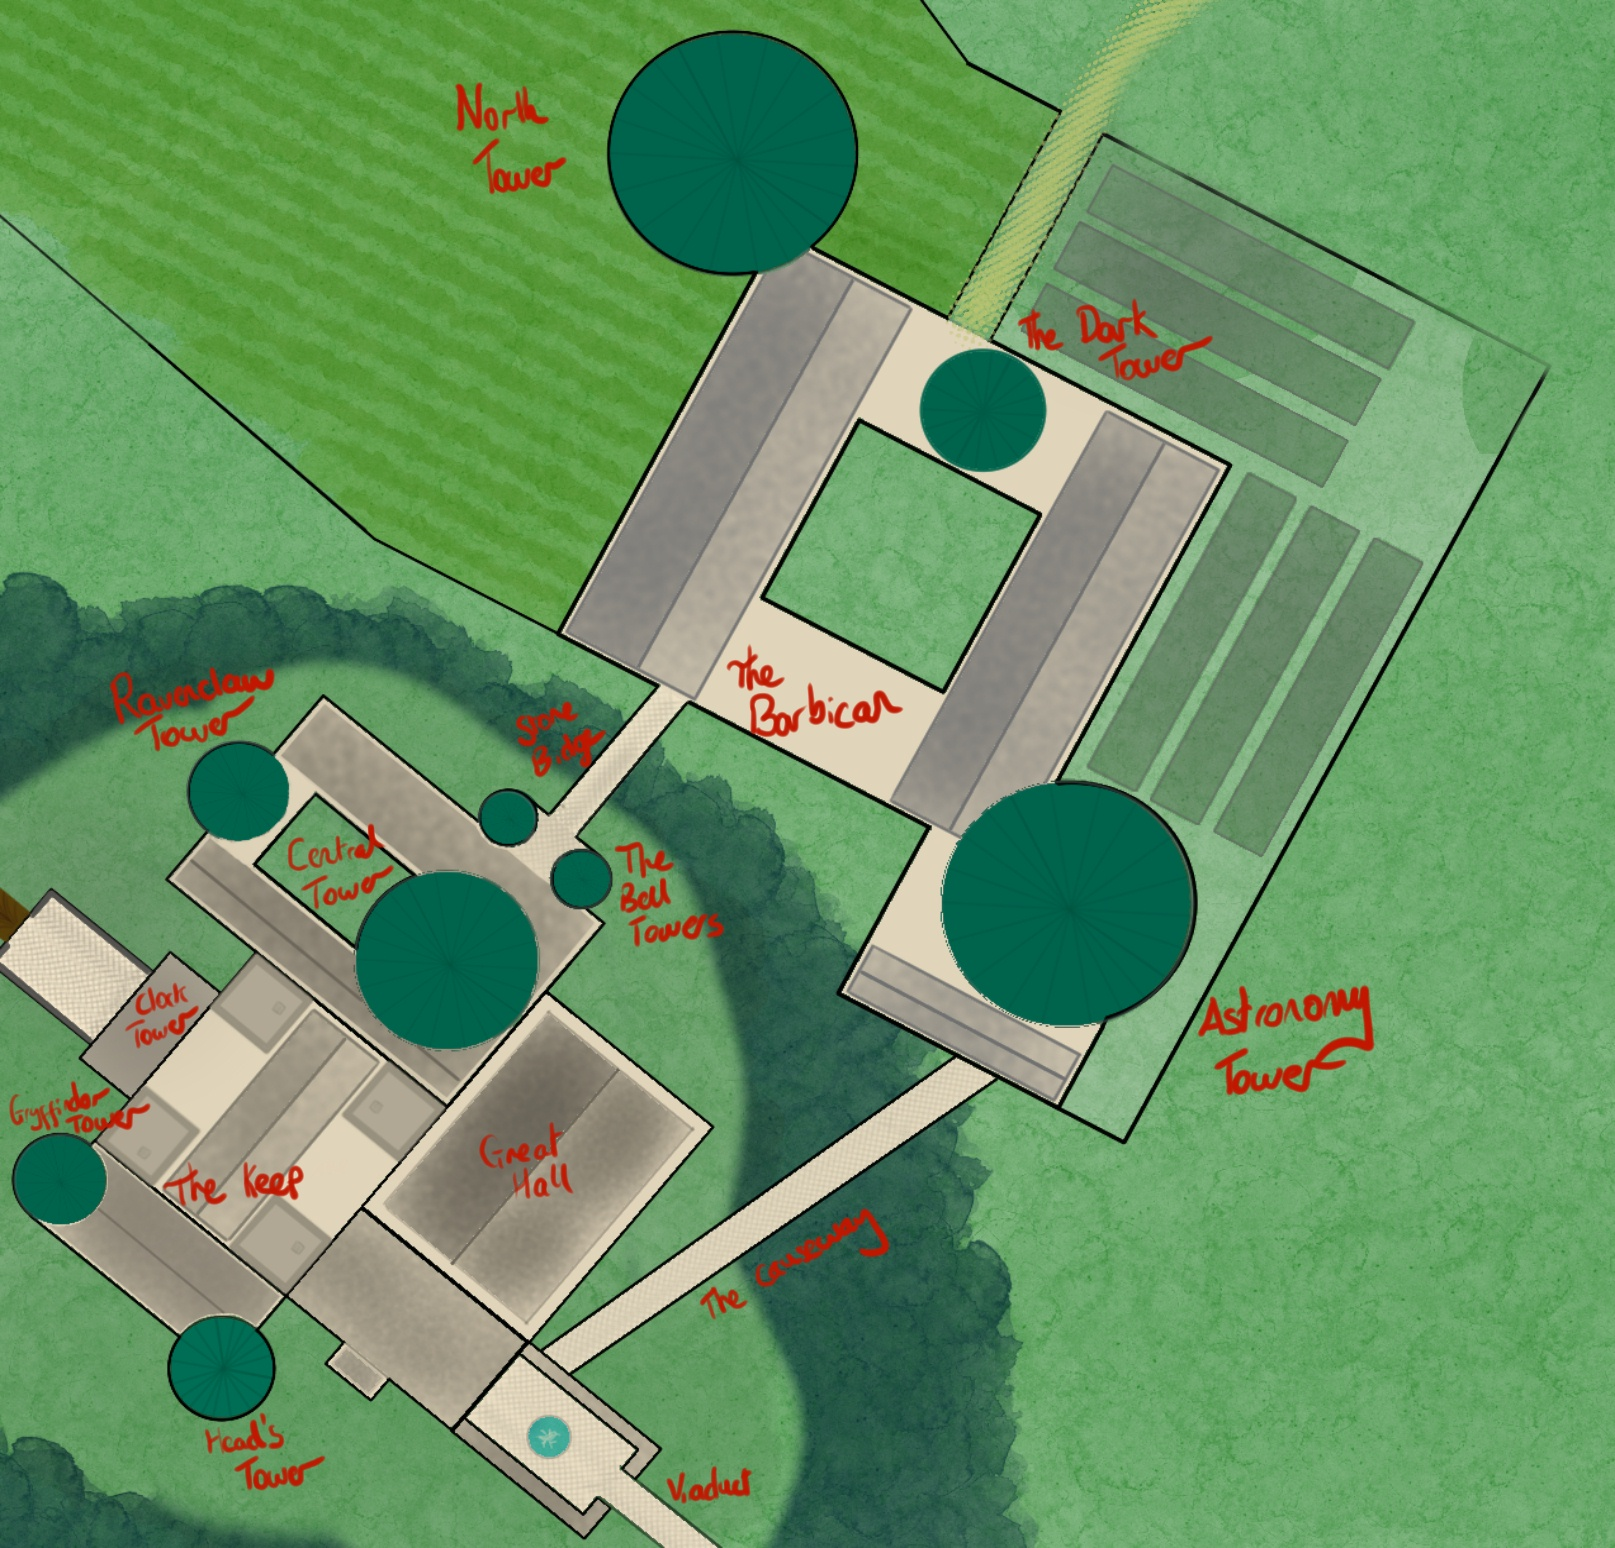
\includegraphics[keepaspectratio = true, width = 0.9\textwidth]{../Images/HogwartsLabelled}
	\end{center}
\end{strip}


\section{Students \& School System}

For most of \imp{Hogwarts} history, it has acted as a \imp{Secondary School}, in the parlance of the British Education system - educating students from the age of 11 to 18, through seven years of study. Along the way they study for two major academic milestones - \imp{Ordinary Wizarding Levels} (O.W.Ls) and the \imp{Nastily Exhausting Wizarding Tests} (N.E.W.T.s) which act as the baseline academic qualifications for their further carer. 



From a RPG perspective, roleplaying as 11 year olds might not be the most appealing prospect - and can certainly the limit the kinds of adventures and storylines you can concoct. 

In order to provide a world where students can have a bit more self-reliance, independence and danger - without feeling like you're going to be killing pre-teens - the following variant rule can be adopted:  

\subsubsection{Optional Rule: Higher Education}

Following the fallout of the \imp{Second Wizarding War}, the Wizarding World entered into a period of deep introspection, asking themselves how they could prevent another such catastrophe from occuring. 

One solution that was floated was to reduce the disparity between the \imp{Muggle World} and the \imp{Wizarding World} - rather than separating students from their non-magical peers at 11, they would remain in school with them until the end of the standard muggle education system - at which point (so the theory goes) they would be mature enough to empathise with muggles, and be able to go on to begin their magical education at \imp{Hogwarts} with a more rounded understanding of the world around them. 

In this scenario, \imp{Hogwarts} acts more akin to a Sixth Form or a University rather than a secondary school (and would also help explain why \imp{Hogwarts} has no mathematics or english classes - or even sex education - necessary to provide basic life skills).

Of course, this solution has been beset with problems - particularly from some of the more obnoxious \imp{pureblood} families, who have either elected to homeschool their children or set up `muggle schools' populated entirely by wizarding children, in order to avoid the integration efforts that this system was put in place to provide. 

\newcommand\building[3]
{
	\subsection{#1}
	
	#2
	
	#3

}
\newcommand\floor[2]
{
	\subsubsection{#1}
	
	#2
}

\newcommand\location[2]
{
	\key{#1}
	
	#2

}

\building{Grounds}{The \imp{Grounds} consist of all of the land outside of \imp{Hogwarts}. The grounds are bounded on two sides by a large stone wall\comma{} but the North and Eastern boundaries of the Grounds lie within the \imp{Forbidden Forest} – the actual extent of the \imp{Grounds} into the \imp{Forbidden Forest} is somewhat murky\comma{} and \imp{Hogwarts} exerts very little control over anything beyond the first few trees.}{

{\location{The Great Lake}{The \imp{Great Lake} (also known as the \imp{Black Lake}) is a very large\comma{} freshwater lake lying within the grounds of \imp{Hogwarts}\comma{} with the majority of the lake lying between \imp{Hogwarts Castle} and \imp{Hogsmeade Station}. The main \imp{Keep} of \imp{Hogwarts} is built on a small island in the \imp{Black Lake}. 

Approximately half a mile across at its widest\comma{} the depths of the Lake have mostly been uncharted – primarily out of respect for the colony of \imp{Merpeople} and the \imp{Giant Squid} which reside in its inky waters.}
\location{The Boathouse}{A small boathouse on the rocky shores of \imp{Hogwarts Isle} which contains the magical boats used to transport the \imp{First Years} across the \imp{Great Lake}. A rugged staircase winds up the cliff\minus{}face up to the \imp{Viaduct Courtyard}.}
\location{Quidditch Pitch}{The Quidditch pitch lies to the North\minus{}East of the \imp{Barbican}\comma{} along the very edge of the \imp{Forbidden Forest}. Oval in shape\comma{} with three sets of raised\comma{} golden hoops at either end\comma{} the pitch is surrounded by 4 enormous towers decorated in the colours of the 4 houses\comma{} from which spectators watch the aerial game.}
\location{Herbology Greenhouses}{Wrapped around the North\minus{}Eastern side of the \imp{Barbican} are a number of long\comma{} narrow Greenhouses\comma{} containing all manner of plants and plant\minus{}like creatures. It is here that students have their practical lessons in \imp{Herbology}\comma{} learning to care for and cultivate magical plants.}
\location{Gamekeeper’s Hut}{}
\location{Animal Pens}{Used for \imp{Care of Magical Creatures} classes}
}
}

\building{Keep}{The \imp{Keep} is the largest building at Hogwarts and\comma{} besides the various towers\comma{} it is also the tallest at a full seven stories tall. The \imp{Grand Staircase} spirals up through the centre of the \imp{Keep} allowing access to the various floors\comma{} which contain a large portion of the teaching rooms. 

The \imp{Keep} has three major entrances and exits – the \imp{Clocktower Courtyard}\comma{} the \imp{Viaduct Courtyard} and the multiple passageways and corridors which lead into the \imp{Central Tower}. Both the \imp{Keep} and the \imp{Central Tower} sit upon a small island close to the shore of the \imp{Great Lake} – access to the rest of the castle and the grounds is ensured through a number of bridges which span the cavernous divides.}{
\floor{Basement}
{\location{Kitchens}{}
\location{Hufflepuff Common Room}{}
}
\floor{Ground Floor}
{\location{Entrance Hall}{}
\location{Great Hall}{}
\location{Viaduct Courtyard}{Part of the main entrance to \imp{Hogwarts Castle}\comma{} the \imp{Viaduct Courtyard} is the first thing most visitors will see\comma{} as it connects the \imp{Viaduct} which crosses the \imp{Great Lake} to the \imp{Entrance Hall}. The \imp{Boathouse}\comma{} where first year students arrive\comma{} is accessed through a steep staircase from this courtyard. The \imp{Viaduct Courtyard} was the site of the final battle between \imp{Harry Potter} and \imp{Lord Voldemort}.}
\location{Clock Tower Courtyard}{}
\location{Causeway}{A long\comma{} narrow bridge which connects the \imp{Viaduct Courtyard} to the \imp{Astronomy Tower}.}
\location{Caretaker’s Office}{}
}
\floor{First Floor}
{\location{Defence Against the Dark Arts Classrooms}{}
\location{History of Magic Classrooms}{}
}
\floor{Second Floor}
{\location{Charms Classroom}{}
\location{House\minus{}Heads Offices}{}
}
\floor{Third Floor}
{\location{Armoury}{A large room lined with suits of armour and weapons – seemingly mostly decorative. If the castle is in danger\comma{} these statues spring into life and will defend the students.}
\location{Charms Office}{}
}
\floor{Fourth Floor}
{\location{Defence Against the Dark Arts Office}{}
}
\floor{Fifth Floor}
{\location{Muggle Studies Classroom}{}
\location{Potions Office (Secondary)}{Not all potions masters appreciate the constant darkness of the \imp{Dungeons}\comma{} even if they are safe for experimentation. \imp{Horace Slughorn} started the tradition of having a second office above ground – something which has continued to this day.}
}
\floor{Sixth Floor}
{\location{Ancient Runes}{}
}
\floor{Seventh Floor}
{\location{Arithmancy Classroom}{}
\location{Room of Requirement}{}
}
\floor{Multiple Floors}
{\location{Grand Staircase}{The \imp{Grand Staircase} is an enormous wood\minus{}pannelled and painting\minus{}covered staircase which runs up vertically through the \imp{Keep}\comma{} covering all seven floors above ground and extending to the \imp{Basement} and the \imp{Dungeons}. 

The most notable feature of the \imp{Grand Staircase} is the fact that the stairs swing backwards and forwards\comma{} pivoting on their axis – allowing students to hop on and hop off as they reach their destination.}
}
}

\building{Central Tower}{The \imp{Central Tower} consists of a large\comma{} low slung building which contains the \imp{Library} and the \imp{Hospital Wing}\comma{} over which the eponymous tower rises. The \imp{Central Tower} is connected to the \imp{Keep} through multiple corridors at the lower levels\comma{} and the \imp{Stony Bridge} allows access to the \imp{Barbican}.}{
\floor{Ground Floor}
{\location{Study Rooms}{A number of large\comma{} brightly lit classrooms where students can go to study. A smaller number of well\minus{}soundproofed and well\minus{} shielded rooms are also provided for students to practice magic in a safe environment.}
\location{Walled Courtyard}{}
}
\floor{First Floor}
{\location{Library: Lower Floor}{}
\location{Stone Bridge}{The \imp{Stone Bridge} is a solidly built bridge protruding from the \imp{Central Tower} across a small part of the \imp{Great Lake}. Aside from the \imp{Causeway} it is the main point of access between the \imp{Barbican} and the rest of the castle.}
}
\floor{Second Floor}
{\location{Library: Upper Floor}{}
\location{Library: Restricted Section}{}
\location{Hospital Wing}{The domain of \imp{Madame Pomfrey}\comma{} the \imp{Hospital Wing}}
}
\floor{Fourth Floor}
{\location{Trophy Room}{A large room dedicated to the trophies and prestigious awards given to students across the years. In the very centre of the room lies the \imp{House Cup}\comma{} adorned in the colours of the current reigning champions.}
}
\floor{Seventh Floor}
{\location{Owlery}{At the very top of the \imp{Central Tower} is a large open space dedicated to the \imp{Owls} of both students and staff to live in.}
}
}

\building{Barbican}{}{
\floor{Ground Floor}
{\location{Transfiguration Courtyard}{}
\location{Transfiguration Classrooms}{}
}
\floor{First Floor}
{\location{Herbology Classrooms}{On some rare occaisions\comma{} \imp{Herbology} classes take a veer into the theoretical\comma{} rather than the practical. When this happens\comma{} they use these classrooms\comma{} which overlook the greenhouses.}
}
\floor{}
{\location{Care of Magical Creatures Classroom}{Some magical creatures are simply too dangerous to let students meet in the \imp{Animal Pens}\comma{} so they are discussed in a more theoretical sense in these classrooms. 

Some of these classrooms have also been converted into habitats for some of the creatures whoa re kept as specimens for these classes\comma{} but who do not enjoy living outdoors.}
}
\floor{Multiple Floors}
{\location{Dark Tower}{The \imp{Dark Tower} is an empty and disused tower which stands above the \imp{Barbican}. The tower was used in years gone by as a prison \minus{} \imp{Sirius Black} was imprisoned here\comma{} as was \imp{Barty Crouch Jnr} – though in modern times it has\comma{} at least officially\comma{} been relegated to storage.}
}
}

\building{North Tower}{The \imp{North Tower} is almost completely freestanding\comma{} towering above and mostly separate from the \imp{Barbican}.}{
\floor{Ground Floor}
{\location{Music Classrooms}{}
}
\floor{First Floor}
{\location{Art Classroom}{}
}
\floor{Second Floor}
{\location{Ancient Studies}{}
}
\floor{Third Floor}
{\location{Magical Theory Classroom}{}
}
\floor{Fourth Floor}
{\location{Recuperative Studies}{}
}
\floor{Fifth Floor}
{\location{Divination Classroom}{}
}
\floor{Sixth Floor}
{\location{Divination Office}{}
}
}

\building{Astronomy Tower}{}{
\floor{First – Sixth floors}
{\location{Staff Quarters}{Much of the lower levels of the \imp{Astronomy Tower} are dedicated to the staff quarters\comma{} where the members of staff live – sometimes with their families. This area is large and spacious\comma{} providing insulated homes amongst areas of indoor greenery – students are generally not allowed within these floors}
}
\floor{Seventh-Eight Floors}
{\location{Astronomy Classrooms}{Unusualy arranged classrooms (which take up a surprising amount of space)\comma{} the astronomy classrooms are arranged in circles with the desks facing outwards – to best give students a view from the expansive windows and into the starry sky.}
}
\floor{Ninth Floor}
{\location{Viewing Platform}{A large flat platform atop the \imp{Astronomy Tower}\comma{} decorated with various bits of telescope apparatus and astrometic devices. It was from this location that \imp{Albus Dumbledore} fell to his death in 1997.}
}
}

\building{Gryffindor Tower}{\imp{Gryffindor Tower} is one of the many towers which juts out from the very top of the \imp{Keep}\comma{} overlooking the rest of the castle. This tower\comma{} as the name suggests\comma{} contains the common room and living quarters associated with \imp{Gryffindor House}. The only access to the tower is hidden behind a portrait of a `fat lady’ on a corridor on the seventh floor.}{

{\location{Gryffindor Common Room}{}
}
}

\building{Ravenclaw Tower}{\imp{Ravenclaw Tower} rises up above the main body of the \imp{Central Tower} (though not as tall as the eponymous tower). The tower houses the living quarters of \imp{Ravenclaw House}\comma{} and in keeping with the teachings of \imp{Ravenclaw}\comma{} the tower can only be accessed by answering a riddle posed by a statue found within the \imp{Library}.}{
}

\building{Dungeons}{Though accessible from the \imp{Grand Staircase} in the \imp{Keep}\comma{} the \imp{Dungeons} sprawl across a much larger region than one might expect\comma{} extending a signifiant distance under the lake.}{

{\location{Slytherin Common Room}{}
\location{Potions Classroom}{}
\location{Potions Office}{}
\location{Potions Storeroom}{}
\location{Chamber of Secrets}{Once only accessible through the Girls Bathroom on the second floor and previously home to the fearsome \imp{Serpent of Slytherin} – a particularly long lived and vicious \imp{Basilisk} – the \imp{Chamber of Secrets} has since been renovated and turned into a practice arena where students can encounter fearsome beasts\comma{} or engage in wizarding duels in a controlled environment.}
}
}

\building{Headmaster’s Tower}{This almost impossibly narrow tower protrudes from the southern edge of the \imp{Keep}\comma{} starting from around the second floor\comma{} where entrance is gained behind a statue of a might golden griffin. The tower itself is almost entirely comprised of a spiral staircase leading to the top of the tower\comma{} where the \imp{Headmaster’s Office} can be found.}{

{\location{Headmaster’s Office}{}
}
}


